
\resetcounters

\bibliographystyle{asp2010}

\markboth{Perez, Vallejo, and Perez}{Migrating an In-Operation Space Observatory Data Processing Chain}

\title{Migrating an In-Operation Space Observatory Data Processing Chain Towards a SOA Oriented Architecture, and the Benefits for Other Space Missions}
\author{Oscar Perez, Juan C. Vallejo, and Ruben F. Perez
\affil{GMV Aerospace and Defence, Isaac Newton 11, Tres Cantos, Madrid, Spain}
}

\aindex{Perez, O.}
\aindex{Vallejo, J.}
\aindex{Perez, R. F.}

\begin{abstract}
The XMM-Newton Science Control System is currently under a migration exercise  aiming to preserve the processing functionality up to the end of the mission, but also to enhance the user accessibility to the different processing and monitoring subsystems. This migration exercise is also providing new insights into how different architectures can help to support other space missions with large demands on processing and storage needs. Service Oriented Architectures and Cloud have also been used in EO missions with results of high interest in storage and processing. In this paper, a prototyping activity is described to face storage and processing in the case of XMM-Newton having in mind its application to other missions with similar needs.    
\end{abstract}

\section{Introduction}
XMM-Newton is an ESA X-ray cornerstone observatory mission, operating continuously with great success since 2000. A continuous migration effort is being done for keeping the processing capabilities of XMM Science Control System (XSCS), in charge of the L0/L1 level products. The main goal is to preserve the processing capabilities along the whole operational lifetime and beyond. It also aims to simplify, modernize and ease the control of the operational data flow. But a third goal is to allow external users and systems to interact with the operational side of the processing. These activities are carried out in coordination with the XSCS Proposal Handling side, the SAS Analysis System and XSA mission archive activities, following a modular ground segment paradigm. Within this abstraction, every module can be migrated using different techniques, different base technologies and different calendar schedules. As a consequence, an in-operations replacement and overhaul of the whole set of subsystems is permitted with no interruption in the data processing flow. A SOA architecture is being implemented for allowing new access and commanding capabilities to the heritage internal core functionality. The processing chain software components are set as individual functionalities with a clear set of defined interfaces. These activities are being carried out sharing synergies with similar projects. In particular, the prototypes developed for cloud services will benefit from GMV modular-SOC studies' conclusions and will offer interesting results to data preservation and processing architectures for Earth Observation (EO) missions. Specifically, the results of these activities could contribute to EO  current studies involving advanced architectures (e.g. Service Oriented Architectures, System of Systems methodologies, etc.). Conversely, these activities in astronomy missions such as XMM-Newton are also addressed when defining EO missions.

\section{XMM-Newton Infrastructure}
Current XMM-Newton Science Control System architecture is showed in Figure~1. It can be divided into downlink and uplink chains. The first chain is mainly in charge of the observation monitoring, raw telemetry processing and L0/L1 products production \citep{vallejo11}. The uplink chain systems are mainly dedicated to the handling of the proposed observations and creation of command sequences which will be later sent to the Mission Operations Center (MOC). Initial design imposed an isolation between both chains, which constrained the operability of the XSCS as a whole. 
\begin{figure}[h]
\centering
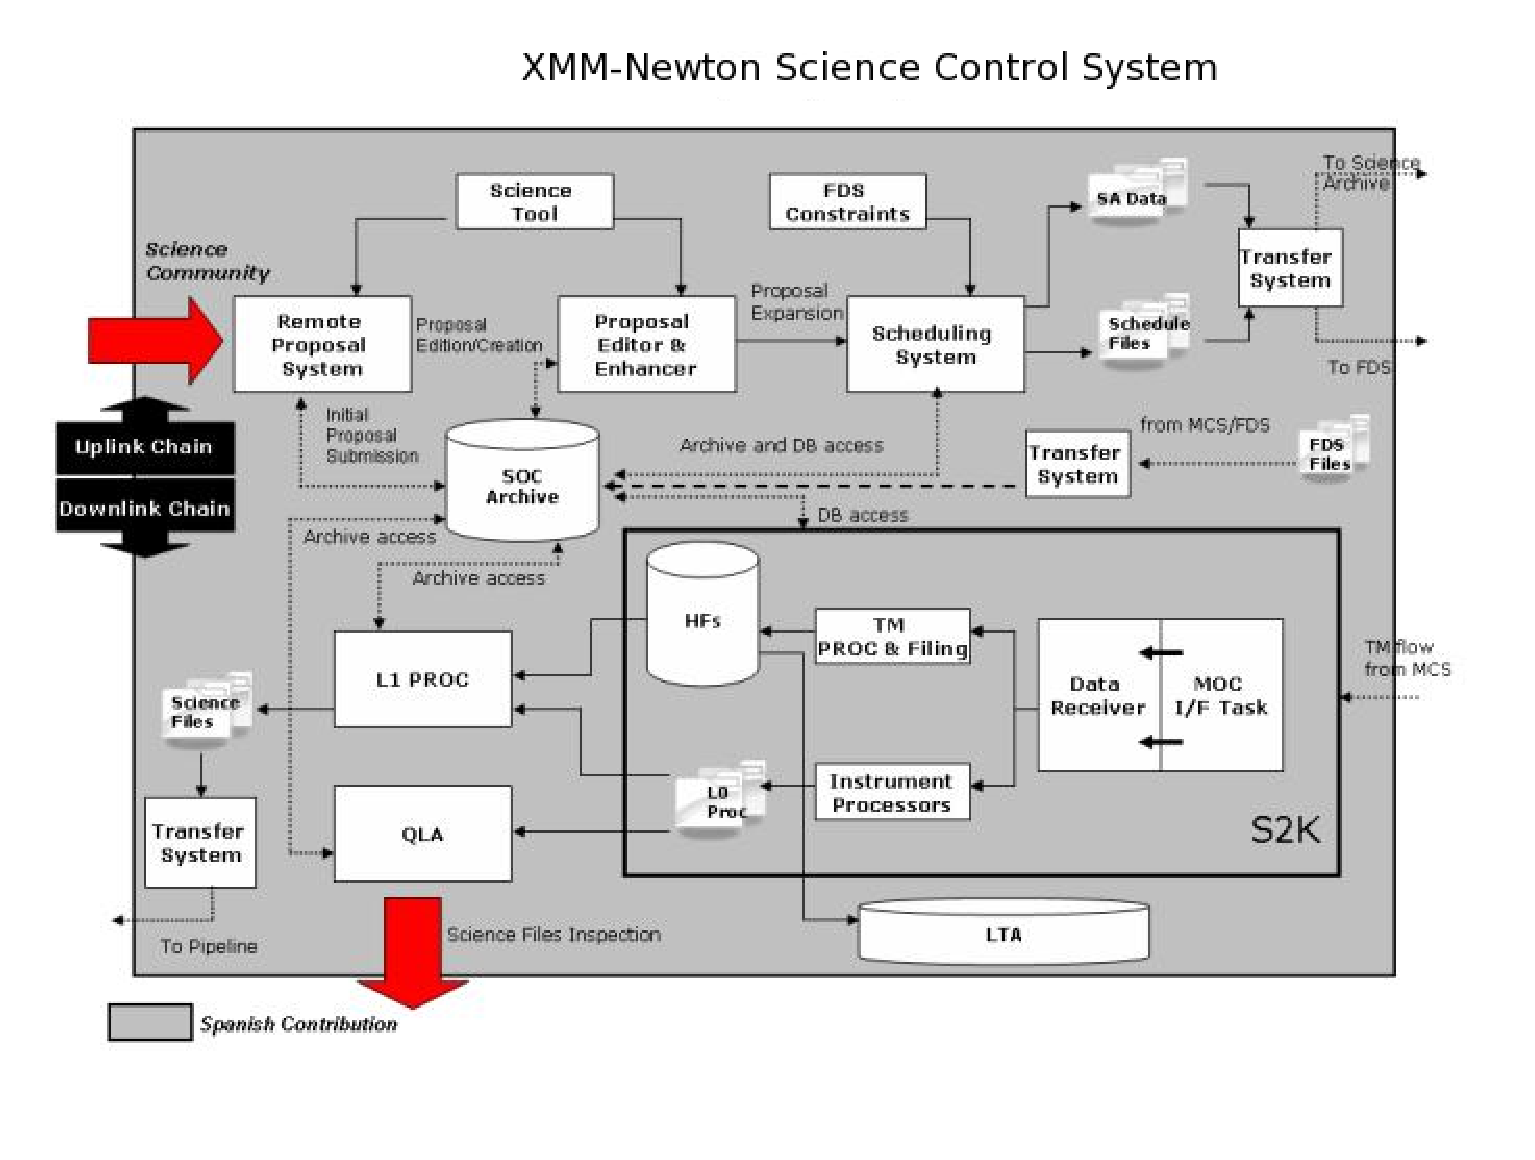
\includegraphics[width=90 mm]{part10/Perez_P022/P022_f1.eps}
\caption{The current XMM-Newton Science Control System (XSCS) architecture}
\label{fig:1}
\end{figure}
Being a long-life mission, the users' needs have evolved with time, the old hardware has been replaced and a migration exercise is on going aiming to simplify the existing data flow structure as much as possible. But what is more important, this migration also aims to improve the operation flexibility to the monitoring and control of the processing and to facilitate an integrated operation of both the downlink and uplink chains. A SOA architecture is expected to achieve this, as both old legacy applications and new user tools may benefit from having flexible ways to access the operational core of the system. 

\subsection{Infrastructure Evolution}
The new infrastructure is to be accord to SOA principles and best practices. The main concepts consist in loosely coupling and component reusability, in order to face a changing business environment. The general idea of SOA is to drive software to a high flexibility, scalability, extensibility, and plug-and-play architecture modifying legacy systems as little as possible \citep{soa1}. Figure 2 depicts the main services envisaged in the scope of the prototype as aligned with the services taxonomy that can be found in the literature \citep{soa2}.
\begin{figure}[h]
\centering
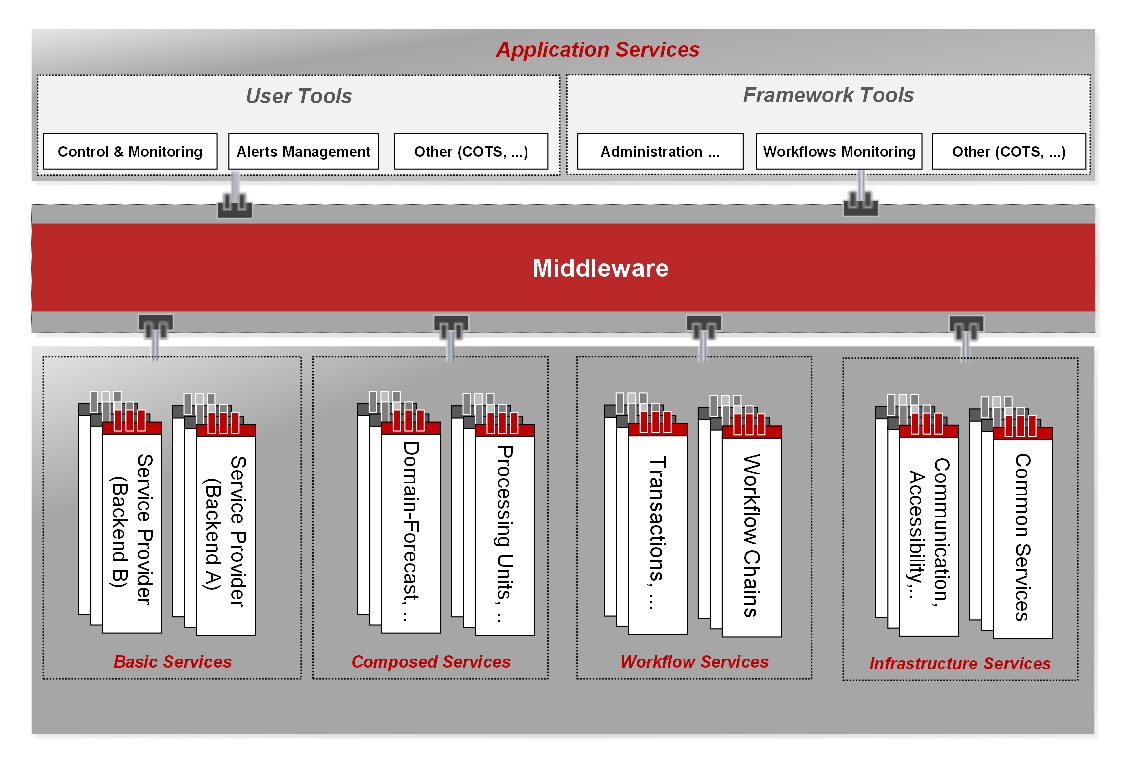
\includegraphics[width=80 mm]{part10/Perez_P022/P022_f2.eps}
\caption{Service Oriented Architecture}
\end{figure}
The middleware represents the way to distribute the data between the different application services of the platform. In many cases, the information is exchanged through pieces (e.g. messages for the case of Message Oriented Middleware) that may be sent to a subject so the subscribed services can receive this information from other services. The implementation of the SOA will be performed from the existing three-tier application architecture. The data access layer represents the very old core of the XSCS, where new handlers and interfaces have been implemented according to the new business logic, which is implemented into the current business layer. The business layer is also enhanced for bridging with the new XSCS presentation layer, where the logic of the services is implemented reusing the infrastructure of existing remote web Proposal Handler facilities. Here is where the most of the service implementation is to take place, as the middleware located here can talk both with the operational side of the processing and monitoring systems, and at the same time, is able to communicate with external entities, either XSCS or non-XSCS based. This is indeed the most relevant aspect of the architecture, as it will offer processing services to non-XSCS external user-driven systems. Thanks to those improvements, the presentation layer will be updated with operational XSCS uplink and downlink (science monitor) systems. But also non-XSCS systems, some of them developed by other SOC parts will manage a broad and updated communication with the core legacy systems. Initial prototyped services are the discovery of new observational L1 product availability and requests for operational archive data. Additional services in the uplink side are status monitoring of observations and remote execution of observation edition facilities. Data flow monitoring tools are common for uplink and downlink. 

\subsection{Storage and Processing Cloud}
In addition to the above, GMV is taking such a scenario as the baseline for studying  new paradigms of having processing infrastructures  able to cope with both the processing of large amounts of data and its storage. These activities  are indeed forming part of a wider exercise in which other projects are under consideration, mainly Earth Observations missions, which have similar processing needs. We focus here in the necessary support to increasing storage and processing capabilities and the associated different policies for distribution among the centers involved in the whole data processing flow, where different studies have been performed by GMV \citep{RubenPerez1}.
\begin{figure}[h]
\centering
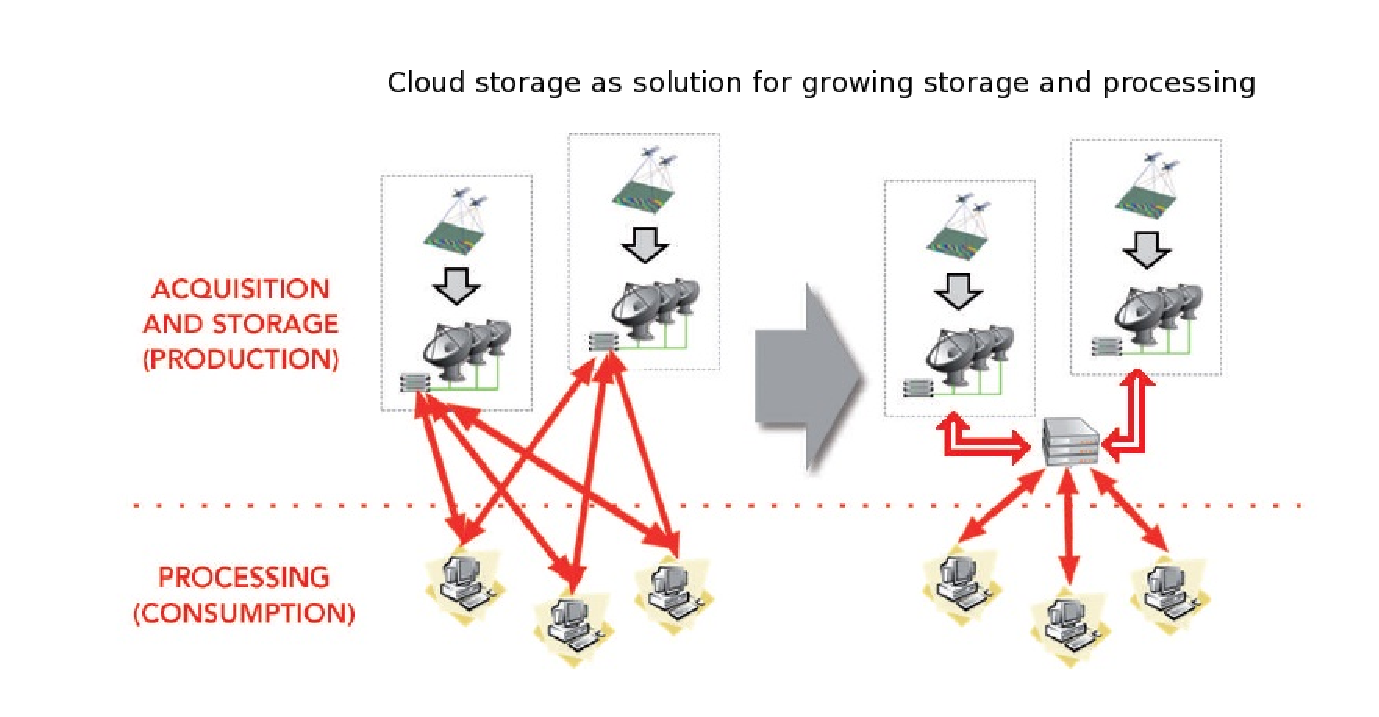
\includegraphics[width=80 mm]{part10/Perez_P022/P022_f3.eps}
\caption{Cloud Processing and Storage in a non centralized environment}

\end{figure}
Different architectures can be deployed to deal with all the data produced by all the missions. In particular, SOA is a perfect architecture to integrate very different systems and perfectly compatible with Cloud in order to maximize extensibility and optimization of computational resources. The architectures being tested are assessed to check two main factors: if current technologies cover the gap between what is required in terms of performance and what the providers currently deliver, and in a second stage, to check if the security provided by external providers fits with the policies of the stakeholders.

At this moment, the architectures being tested are:
\begin{itemize}
\item Private cloud, to provide horizontal accessibility and discoverability where the main elements are a file Viewer (to identify the files location by ESA), a Search Engine (to be used by the Community Users), and a Curation Tool (which allows the different authorized users to insert/read metadata).
\item Public cloud: where what really needs to be checked is if it is feasible to outsource storage and processing to a Centre which uses Cloud Computing while keeping the same accessibility and discoverability offered in the first architecture. This architecture takes advantage of the horizontal accessibility, but adding the complexity of using a Cloud to perform the outsourcing.
\end{itemize}

In both solutions, an IaaS (Infrastructure as a Service), Paas (Platform as a Service) and SaaS (Software as a Service) in the cloud are preferred, since the end user not only wants to use the platform to run their processing algorithms to check if the final products improve with their assumptions, but also wants to run the applications provided by the client to analyze the data.

\bibliography{editor}
